\section{Introduction}

Quantum sensors, being strongly sensitive to external disturbances, are able to measure various physical phenomena with extreme sensitivity.
These quantum sensors interact with the environment and have the environment phenomenon or parameters encoded in their state~\cite{RevModPhys.quantumsensing}.
A group of distributed quantum sensors, if prepared in an appropriate entangled state, can further enhance the estimation of a single continuous parameter, improving the standard deviation of measurement by a factor of $1/\sqrt{m}$ for $m$ sensors (Heisenberg limit)~\cite{Giovannetti_2011}.
\eat{Recently, experimental physicists successfully demonstrated a reconfigurable distributed radio-frequency photonic sensor network~\cite{PRL20-qsn,arizona21-thesis} that utilizes squeezed quantum state and entanglement to enhance sensing of radio signals.}
% The experiments establish a connection between the entanglement structure and the achievable quantum advantage in different distributed sensing problems.

Recently, many protocols have been developed for the estimation of a single 
parameter or multiple independent parameters~\cite{Giovannetti_2011,Proctor_2018} using one or multiple (possibly, entangled) sensors. 
But, the use of a distributed set of quantum sensors working collaboratively 
to estimate more complex physical/environmental phenomena, as in many classical
sensor network applications~\cite{tsn17-water, sensys10-health,mobicom03-sensor}, 
has not been explored much.
% In this paper, we develop a scheme for the localization of events using a quantum sensor network (QSN);
In this paper, we explore a potential quantum sensor network application--- localization of events.
In particular, we develop effective techniques 
for radio frequency (RF) transmitter localization and thus demonstrate the promise of QSNs in the accurate localization of events. Our motivation for choosing 
RF transmitter localization as the event localization 
application is driven by the significance of transmitter localization
in  wireless/mobile applications and recent advances in quantum sensor
technologies for RF signal detection (see \S\ref{sec:problem}).

\begin{figure*}[t]
    \centering
    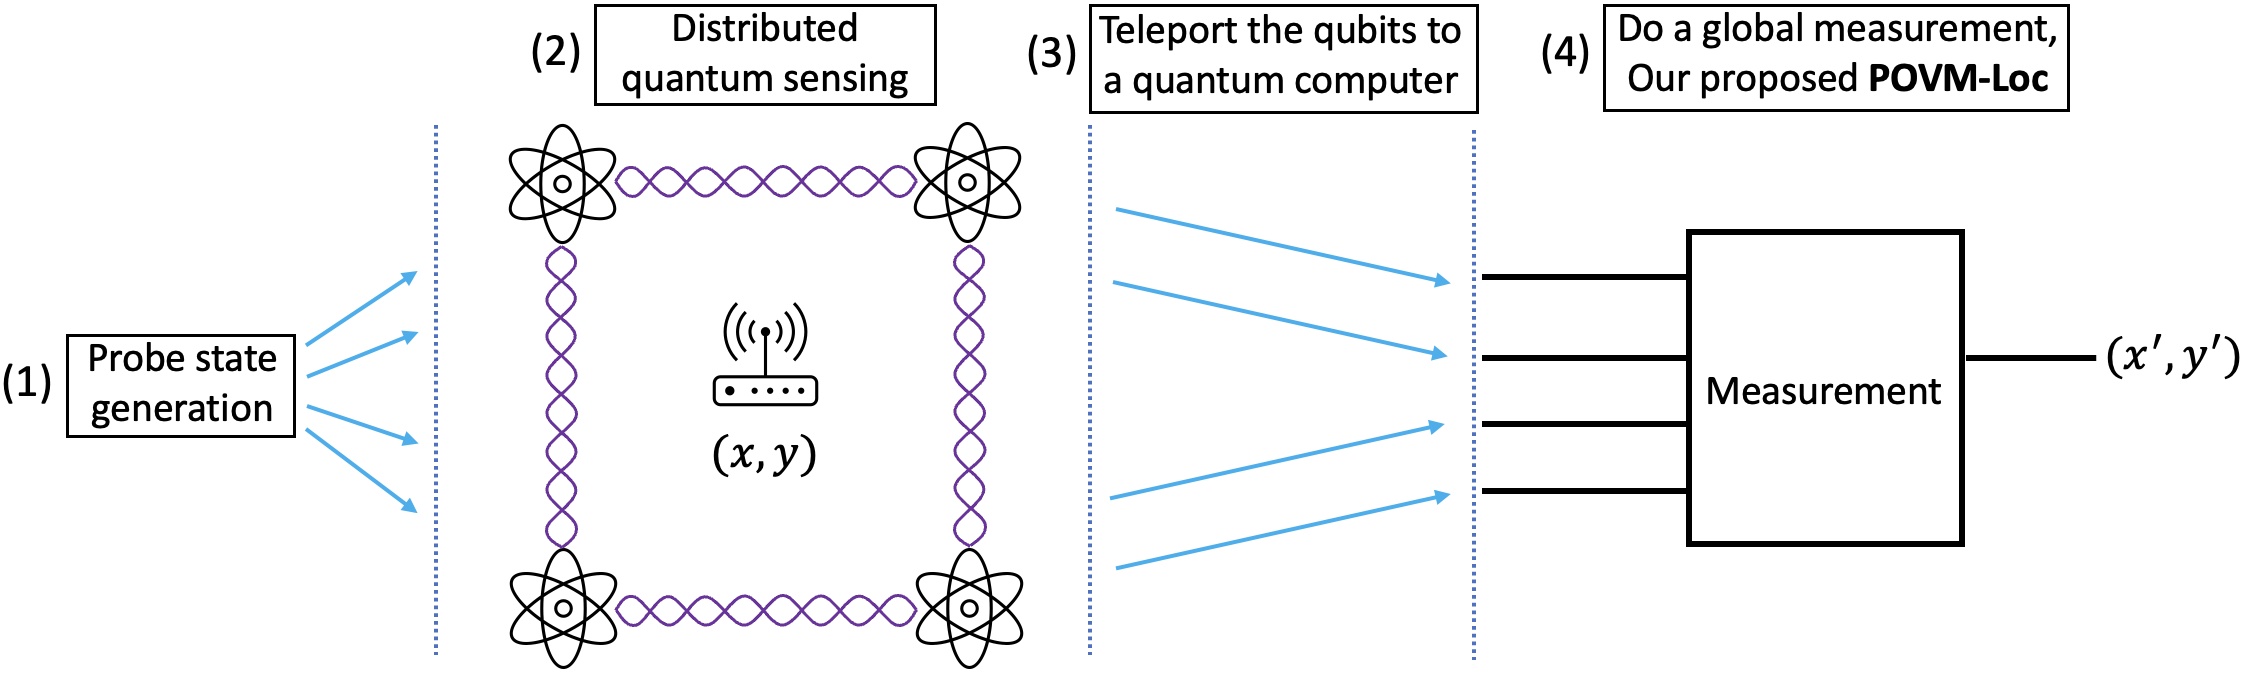
\includegraphics[width=0.95\textwidth]{chapters/qce/figures/overall.png}
    %\vspace{-0.1in}
    \caption{Overall architecture of using a QSN to localize a transmitter. 
    % The transmitter's location is at $(x, y)$ and the estimated location is $(x', y')$
    }
    \label{fig:quantumoverall}
\end{figure*}

\para{Transmitter Localization using QSNs.}
Our approach to
transmitter localization using QSNs essentially involves posing
the localization problem as a quantum state discrimination
(QSD) problem~\cite{bergou-review-2007} which is to identify the specific state a given
quantum state is in (from a given set of states in which the
system can be) by performing quantum measurements on the
given quantum system. The overall architecture is illustrated in
Fig.~\ref{fig:quantumoverall}. 
First, a probe state is generated and distributed to the
QSN. Then, once the quantum sensors have been impacted
(i.e., the overall quantum state changed) due to the transmission
from the transmitter’s signal, an appropriate quantum measurement 
is made on the quantum state of the network.
The outcome of the measurement determines the quantum
state, and thus, the location of the transmitter. 
However, the
above process can be erroneous, as solving 
the QSD problem even optimally
can incur a certain probability of (classification/discrimination)  error.
This paper’s goal is to develop an approach with a 
minimal localization error. 
%%%%%%%%%
In that context, our
developed schemes in this paper are based on two ideas that extend
the above basic QSD-based approach: 
\begin{enumerate}
    \item We use a two-level approach
that localizes the transmitter in two stages: first, at a coarse level
using a set of sensors over the entire area, and then, at a fine level
within the ``block'' determined by the first level. 
\item In addition, we circumvent the challenge of implementing a general
measurement operation, by instead using a trained parameterized 
hybrid quantum-classical circuit that essentially implements the 
measurement operation and predicts the transmitter location from
quantum sensor data.
\end{enumerate}
Our evaluation results show that our best scheme (which combines the above two ideas) is able to achieve meter-level (1-5m) localization accuracy; in case of discrete locations, it achieves near-perfect (99-100\%) classification accuracy. 

\para{Contributions.} 
In the above context, we make the following contributions. 
\begin{enumerate}
    \item We model the transmitter localization problem as a well-studied quantum state discrimination (QSD) problem, which allows us to develop viable transmitter localization schemes using quantum sensors. 
 
    \item 
    We design two high-level schemes to localize a transmitter in a given area deployed with a quantum sensor network.
     The first scheme is based on solving an appropriate quantum state discrimination problem using a global measurement, while the second scheme uses a trained hybrid quantum-classical circuit to process the quantum sensor data. Within the above high-level schemes, we also introduce a two-level localization scheme to improve the performance of the basic one-level schemes.
  
    \item 
    To evaluate our schemes, we model how a quantum sensor's state evolves due to RF signals from a transmitter at a certain distance. Using this model, we 
     evaluate our localization schemes and demonstrate their effectiveness in our custom-built simulator.
\end{enumerate}

% \magenta{To the best of our knowledge, ours is one of the two recent works to investigate and develop techniques for event-localization problems using a collaborative 
% network of quantum sensors. 
% The other work is~\cite{PR22-quantum_positioning} who uses a small network of four quantum sensors to localize an incoming signal by estimating the signal's angle of arrival to different sensors.
% ~\cite{PR22-quantum_positioning} introduced the concept, however, they didn't evaluate their methods and didn't provide specific localization error numbers.
% We take a different route by using quantum sensors that are impacted by the signal's strength, instead resorting to arriving angles.
% Also, we are able to show the effectiveness of our proposed methods through extensive simulated experiments.}

\para{Paper Organization.} The paper is organized as follows. 
In \S\ref{sec:problem}, we present our quantum sensor model, formally define the transmitter localization problem and discuss related work.
In the following two sections, we describe our two classes of algorithm: quantum-state-discrimination (QSD) based scheme, and parameterized-quantum-circuit (PQC) based scheme.
We discuss our evaluation results in \S\ref{sec:eval}, and give concluding remarks
in \S\ref{sec:conclusion}.